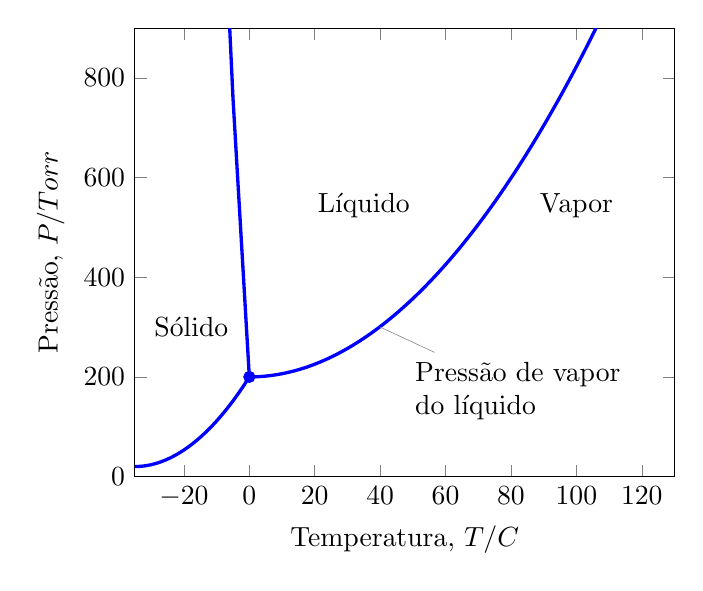
\begin{tikzpicture}
\begin{axis}
        [
            grid = minor,
            ylabel = {Pressão, $P/\unit{Torr}$},
            xlabel = {Temperatura, $T/\unit{\degree C}$},
            ymin=0, ymax=900,
            xmin=-35, xmax=130,
        ]       
        \draw [draw=blue, very thick]
            (axis cs: -35, 20) parabola 
            (axis cs: 0, 200);
        \draw [draw=blue, very thick]
            (axis cs: 0, 200) --
            (axis cs: -5, 760) --
            (axis cs: -6, 900);
        \draw [draw=blue, very thick]
            (axis cs: 0, 200) parabola
            (axis cs: 120, 1100);

        \addplot [ mark=*, color=blue, only marks ] coordinates
            { 
                (0, 200)
            };

        \node [anchor = west, align = center] at (axis cs:-32, 300) 
            { Sólido };

        \node [anchor = south] at (axis cs:35, 500) 
            { Líquido };

        \node [anchor = south] at (axis cs:100, 500) 
            { Vapor };

        \node[coordinate, pin={[fill=white, align=left] below right:{Pressão de vapor \\do líquido}}] 
            at (axis cs:40,300)   {};
\end{axis}
\end{tikzpicture}